\chapter{状态估计}
\section{基础理论知识}
本节主要参考了文献\texttt{State Estimation for Micro Air Vehicles}的第4、5节内容。
\subsection{低通滤波器}
低通滤波器可以认为是一种较为简单的估计器。常见的一阶低通滤波器可以表示为:
\begin{equation*}
    Y(s) = \frac{a}{s+a}U(s)
\end{equation*}
通过Laplace逆变换可以得到时域形式为:
\begin{equation}
    \dot{y} = -ay+au
\end{equation}
进一步地,求解该微分方程可得:
\begin{equation*}
    y(t+T) = e^{-aT}y(t) + a\int_0^T{e^{-a(T-\tau)}u(\tau)}\dd{\tau}
\end{equation*}
如果用$T_s$表示采样周期,且假设$u(t)$在采样周期内保持常值,那么有:
\begin{align}
    y(k+1) & = e^{-a T_s} y(k) + a \int_0^{T_s}{e^{-a(T_s-\tau)}}\dd{\tau} \cdot u(k) \notag \\
    & = e^{-aT_s} y(k) + (1-e^{-aT_s}) u(k)
\end{align}
定义$\alpha_{LPF} = e ^ {-a T_s}$,则可以进一步简化为:
\begin{equation}
    y(k+1) = \alpha_{LPF} y(k) + (1-\alpha_{LPF}) u(k)
\end{equation}
如果用符号$LPF(\cdot)$表示上述的低通滤波运算,那么$\hat{x} = LPF(x)$就是$x$在低通滤波下的估计值。

\subsection{动态观测器}
考虑一个LTI系统并表示为:
\begin{align*}
    \dot{x} & = A x + B u \\
    y & = C x
\end{align*}
对于该系统的连续时间观测器可以表示为:
\begin{equation}
    \dot{\hat{x}} = A \hat{x} + B u + L(y-C\hat{x})
\end{equation}
其中,$\hat{x}$为$x$的估计值。上式中等号右端前两项可以认为是对原系统的预估,最后一项可以认为是利用观测数据对状态的校正。定义估计误差为$\tilde{x} = x - \hat{x}$,那么可以得到:
\begin{equation}
    \dot{\tilde{x}} = (A - L C)\tilde{x}
\end{equation}
这表明如果选择合适的$L$值使得矩阵$A-LC$是Hurwitz稳定的,那么估计误差将以指数方式收敛到零。

如果观测数据并不是在每一拍都可以获得(传感器数据更新较慢),那么可以采用如下的两步方式进行处理,如图\ref{fig: estimator1}所示。

在没有得到传感器数据的时候,只使用预估方式进行估计:
\begin{equation}
    \dot{\hat{x}} = A \hat{x} + B u    
\end{equation}
当得到传感器数据后,则进行校正:
\begin{equation}
    \hat{x}^+ = \hat{x}^- + L(y(t_k) - C \hat{x}^-)
\end{equation}
其中,$\hat{x}^-$表示预估值,$\hat{x}^+$表示校正值。注意到,在这种处理方式下,并不要求传感器数据以固定频率更新。
\begin{figure}[htbp]
	\figskip
	\centering
	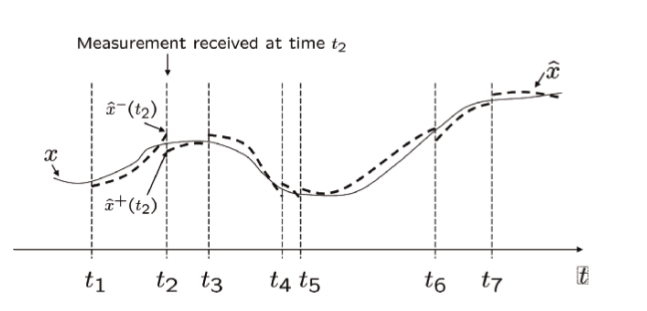
\includegraphics[width = 0.6\textwidth,trim = 0 -0 0 -0,clip]{estimator1.png}	  
	\caption{\label{fig: estimator1} 用动态观测器进行预估-校正方式的状态估计}
\end{figure} 

\subsection{连续--离散卡尔曼滤波器}
考虑如下的系统:
\begin{align}
    \dot{\bm{x}} &= \bm{A} \bm{x} + \bm{B} \bm{u} + \bm{\xi} \notag \\
    \bm{y}_k &= \bm{C} \bm{x}_k + \bm{\eta}_k
\end{align}
其中,状态方程用连续形式表示,观测方程则用离散的形式表示,下标$k$表示第k次采样。
$\bm{\xi}$表示过程噪声,假设均值为0、协方差为$\bf{Q}$,实际中$\bf{Q}$往往是未知的。
$\bm{\eta}_k$表示测量噪声,与传感器特性相关,假设其均值为0、协方差为$\bf{R}$,实际中可以通过传感器标定估计出$\bf{R}$。

那么针对该系统,可以构造与动态观测器形式类似的连续--离散卡尔曼滤波器:
\begin{align}
    \dot{\hat{\bm{x}}} &= \bm{A} \hat{\bm{x}} + \bm{B} \bm{u} \notag \\
    \hat{\bm{x}}^+_k &= \hat{\bm{x}}^-_k + \bm{L} (\bm{y}_k - \bm{C} \hat{\bm{x}}^-_k)
\end{align}

定义滤波器的估计误差$\tilde{\bm{x}} = \bm{x} - \hat{\bm{x}}$,那么估计误差的协方差可以表示为:
\begin{equation}
    \bm{P}(t) = E\left\{ \tilde{\bm{x}}(t) \tilde{\bm{x}}(t)^\uT \right\}
\end{equation}
显然$\bm{P}(t)$是一个对称、半正定的,所以它的特征值均非负。当$\bm{P}(t)$具有较小的特征值时,滤波器估计误差的方差较小,所以这时估计误差也较小。
考虑到
\begin{equation*}
    \rm{tr}(\bm{P}) = \sum{\lambda_i}
\end{equation*} 
{\color{red}所以卡尔曼滤波器就是求解$\bm{L}$使$\rm{tr}(\bm{P})$取得最小值,从而获得在均方误差最小指标下的最优状态估计。}

\noindent {\hei $\blacksquare$ 传感器数据更新前}

对估计误差求导可得:
\begin{align*}
    \dot{\tilde{\bm{x}}} &= \dot{\bm{x}} - \dot{\hat{\bm{x}}} \\
    &= \bm{( Ax+Bu+\xi) - (A\hat{x} + Bu) } \\
    &= \bm{A \tilde{x} + \xi}
\end{align*}
该微分方程的解为:
\begin{equation}
    \bm{\tilde{x}}(t) = e^{\bm{A} t} \tilde{\bm{x}}_0 + \int_0^t{e^{\bm{A} (t-\tau)} \bm{\xi}(\tau)}\dd \tau
\end{equation}
对$\bm{P}$求导可得:
\begin{align*}
    \dot{\bm{P}} &= \D{}{t} E\{\bm{\tilde{x} \tilde{x}^\uT} \} \\
    &= E\{\bm{\dot{\tilde{x}} \tilde{x}^\uT} + \tilde{x}\dot{\tilde{x}}^\uT \} \\
    &= E\{\bm{ A \tilde{x} \tilde{x}^\uT  + \xi\tilde{x}^\uT + \tilde{x}\tilde{x}^\uT A^\uT + \tilde{x} \xi^\uT   } \} \\
    &= \bm{A P + P A^\uT} + E\{ \bm{\xi \tilde{x}^\uT}\} + E\{ \bm{\tilde{x} \xi^\uT} \}
\end{align*}
其中,
\begin{align*}
    E \{ \bm{ \xi \tilde{x}^\uT } \} &= E \left\{ \bm{\xi}(t) \tilde{\bm{x}}_0 e^{\bm{A}^\uT t} 
    + \int_0^t{ \bm{\xi}(t)\bm{\xi}^\uT (\tau) e^{\bm{A}^\uT (t-\tau)} }\dd \tau \right\} \\
    &= \frac 1 2 \bm{Q}
\end{align*}
代入上式可得:
\begin{equation}
    \bm{\dot{P} = A P + P A^\uT + Q}
\end{equation}

\noindent {\hei $\blacksquare$ 传感器数据更新时}

在传感器数据更新时,有:
\begin{equation*}
    \hat{\bm{x}}^+_k = \hat{\bm{x}}^-_k + \bm{L} (\bm{y}_k - \bm{C} \hat{\bm{x}}^-_k)
\end{equation*}
假定$\bm{\eta}$和$\bm{x}$是独立的,也就是$E\{ \tilde{\bm{x}}^- \bm{\eta}^\uT L^\uT  \} = E\{\bm{ L\eta\tilde{x}^{-\uT} }\} = \bm{0}$,那么可以计算$\bm{P}^+$为:
\begin{align}{\label{equ: p+}}
    \bm{P}^+ =& E\{ \tilde{\bm{x}}^+ \tilde{\bm{x}}^{+\uT}   \} \notag \\
            =& E\left\{ \bm{ (\tilde{x}^- - LC\tilde{x}^- - L\eta) (\tilde{x}^- - LC\tilde{x}^- - L\eta)^\uT } \right\}  \notag \\
            =& E\left\{\bm{ \tilde{x}^- \tilde{x}^{-\uT} - \tilde{x}^- \tilde{x}^{-\uT} C^\uT L^\uT - \tilde{x}^- \eta^\uT L^\uT}  \right. \notag \\
            & \bm{ - LC\tilde{x}^- \tilde{x}^{-\uT} + LC \tilde{x}^- \tilde{x}^{-\uT} C^\uT L^\uT + LC\tilde{x}^- \eta^\uT L^\uT}  \notag \\
            & \left. \bm{ - L \eta \tilde{x}^{-\uT} + L \eta \tilde{x}^{-\uT} C^\uT L^\uT + L \eta \eta^\uT L^\uT } \right\}  \notag \\
            =& \bm{ P^- - P^- C^\uT L^\uT - LCP^- + LCP^-C^\uT L^\uT + LRL^\uT }
\end{align}
为了求解使$\rm{tr}(\bm{P}^+)$最小化时的$\bm{L}$值,一个必要的条件为:
\begin{gather*}
    \Q{}{\bm{L}} \rm{tr}(\bm{P}^+) = \bm{-P^- C^\uT - P^- C^\uT + 2LCP^-C^\uT + 2LR} = 0 \\
    \Rightarrow 2 \bm{L(R + CP^-C^\uT)} = 2 \bm{P^-C^\uT} \\
    \Rightarrow \bm{L} = \bm{P^- C^\uT(R+CP^-C^\uT)^{-1}}
\end{gather*}
推导中用到以下矩阵关系:
\begin{gather*}
    \Q{}{\bm{A}} \rm{tr}(\bm{BAD}) = \bm{B^\uT D^\uT} \\
    \Q{}{\bm{A}} \rm{tr}(\bm{ABA^\uT}) = 2 \bm{AB},\,\bm{B} = \bm{B}^\uT
\end{gather*}
将$\bm{L}$的计算式代入式(\ref{equ: p+})中可得:
\begin{equation}
    \bm{P}^+ = \bm{(I - LC)P^-}
\end{equation}

\noindent {\hei $\blacksquare$ 总结}

综合上述推导可以得到如下的卡尔曼滤波器迭代计算公式:
\begin{align*}
     \dot{\hat{\bm{x}}} &= \bm{A \hat{x} + B u} \\
     \dot{\bm{P}} &= \bm{A P + P A^\uT + Q} \\
     \bm{L}_k &= \bm{P^-_k C^\uT(R+CP^-_k C^\uT)^{-1}} \\
     \bm{P}^+_k &= \bm{(I - L_k C)P^-_k} \\
     \hat{\bm{x}}^+_k &= \hat{\bm{x}}^-_k + \bm{L}_k (\bm{y}_k - \bm{C} \hat{\bm{x}}^-_k)
\end{align*}

\subsection{从概率角度的理解}
本节参考自
\href{http://www.bzarg.com/p/how-a-kalman-filter-works-in-pictures/}{\texttt{How a Kalman filter works, in pictures}}
这篇文章。

正态分布的概率密度函数可以表示为:
\begin{equation*}
    N(x,\mu, \sigma) = \frac{1}{\sigma \sqrt{2 \pi}} e^{-\frac{(x-\mu)^2}{2\sigma^2}}
\end{equation*}
对于两个正态分布的随机变量相乘,则有: 
\begin{equation*}
    N(x,\mu_0, \sigma_0) \cdot N(x,\mu_1, \sigma_1) = N(x,\mu', \sigma')
\end{equation*}
其中,相乘后概率分布的参数为:
\begin{equation*}
    \mu' = \frac{\mu_1 \sigma_0^2 + \mu_0 \sigma_1^2}{\sigma_0^2 + \sigma_1^2} = \mu_0 + \frac{\sigma_0^2(\mu_1 - \mu_0)}{\sigma_0^2 + \sigma_1^2}
\end{equation*}
\begin{equation*}
    \sigma' = \frac{\sigma_0^2 \sigma_1^2}{\sigma_0^2 + \sigma_1^2} = \sigma_0^2 - \frac{\sigma_0^4}{\sigma_0^2 + \sigma_1^2}
\end{equation*}

若定义参数$k$为
\begin{equation*}
    k = \frac{\sigma_0^2}{\sigma_0^2 + \sigma_1^2}
\end{equation*}
则有:
\begin{equation*}
    \mu' = \mu_0 + k(\mu_1 - \mu_0)
\end{equation*}
\begin{equation*}
    \sigma' = \sigma_0^2 - k\sigma_0^2
\end{equation*}





\subsection{更多讨论}
以下再讨论几点不一样的地方。

\noindent {\hei $\blacksquare$ 非线性模型和EKF}

若系统动态及测量模型都是非线性的:
\begin{align*}
    \dot{\bm{x}} &= \bm{f}(\bm{x}, \bm{u}) + \bm{\xi} \\
    \bm{y}_k &= \bm{h}(\bm{x}_k) + \bm{\eta}_k
\end{align*}
仍可以通过以下的处理方式,求取非线性函数的雅可比矩阵作为$\bm{A}$、$\bm{C}$:
\begin{align*}
    \bm{A} &= \Q{\bm{f}}{\bm{x}}(\hat{\bm{x}}, \bm{u}) \\
    \bm{C} &= \Q{\bm{h}}{\bm{x}}(\hat{\bm{x}}, \bm{u})
\end{align*}

\noindent {\hei $\blacksquare$ 状态转移矩阵形式的KF}

若系统动态方程用状态转移矩阵的形式表示:
\begin{align*}
    \bm{x}_{k+1} &= \bm{\Phi}(T_s) \bm{x}_k + \bm{G}(T_s) \bm{u}_k 
\end{align*}
其中,
\begin{align*}
    \bm{\Phi}(T_s) &= \bm{\Phi}(t)|_{t=k T_s} = e^{\bm{A} t}|_{t=k T_s} \\
    \bm{G}(T_s) &= \int_0^{T_s}{\bm{\Phi}(\tau) \bm{B}}\dd \tau
\end{align*}
那么这种情况下的卡尔曼滤波器的预测方程应表示为:
\begin{align*}
    \bm{x}_{k+1} &= \bm{\Phi}(T_s) \bm{x}_k + \bm{G}(T_s) \bm{u}_k \\
    \bm{P}_{k+1} &= \bm{\Phi}(T_s) \bm{P}_k^+ \bm{\Phi}^\uT(T_s) + \bm{Q}
\end{align*}

\section{四元数}
本节内容主要参考文献\href{attachment/Quaternion and Rotation.pdf}{\texttt{Quaternion and Rotation}}
\subsection{四元数基本计算}

\subsection{四元数微分方程}
\begin{theorem}
    假设$q(t)$表示一单位四元数函数,$\omega(t)$表示由$q(t)$确定的角速度。那么$q(t)$的导数为:
    \begin{equation*}
        \dot{q} = \frac 1 2 \omega q
    \end{equation*}
\end{theorem}
具体证明可以看参考文献。在实际运动过程中,获得的角速度矢量通常时在旋转坐标系下描述的(如在无人机转动时的机体系下,由三轴陀螺仪获得的角速度)。假设该角速度为$\omega '$,则有$\omega ' = q^*\omega q$。将$\omega = q \omega ' q^*$待如到上述定理中有:
\begin{equation*}
    \dot{q} = \frac 1 2 q \omega '
\end{equation*}


\section{PX4状态估计源码分析}
\subsection{\texttt{attitude_estimator_q}}
通过阅读源码,可以将该状态估计的核心算法归纳如下:
\begin{align*}
    \bm{\delta} &= K_P \bm{e} + K_I \int \bm{e} \\
    \bm{\omega}^+ &= \bm{\omega}^- + \bm{\delta} \\
    \dot{\hat{\bm{q}}} &= \frac 1 2 \hat{\bm{q}} \times \bm{\omega}^+
\end{align*}
其中,$\bm{e}$表示对姿态估计的角度偏差,$\bm{\delta}$表示对角速度的零偏修正量,
$\bm{\omega}^-$表示陀螺读数,$\bm{\omega}^+$表示修正后的角速度。

\setfnsymbol{bringhurst}

可以看出,该算法的核心思想就是将状态估计的{\color{red}所有误差}均视为一个{\color{red} 动态变化的角速度(陀螺读数)零偏值},然后利用PI的方式计算该动态零偏值,并在{\color{red}角速度环}进行修正\footnote{若单纯从角度、角速度、PI控制来理解,会觉得修正量因该补偿在角度上。但是如果联想到ADRC的{\color{red}动态补偿}思想,该算法也有异曲同工的地方。},最后通过积分获得对四元数的状态估计值。

角度偏差$\bm{e}$主要是通过加速度计和磁罗盘进行计算的:利用磁罗盘读数和当前姿态计算地磁偏差,从而获得姿态的偏航误差;利用加速度计及计算的运动加速度,求得重力加速度并计算姿态偏差;最后将两个偏差向量(三轴角度偏差向量)按权重求和。



